% !TeX root = ../tfg.tex
% !TeX encoding = utf8

\chapter{Aprendizaje Automático y Aprendizaje Profundo}\label{ch:capitulo-aprendizaje-automatico-y-profundo}

\section{Fundamentos}\label{sec:fundamentos-aprendizaje-automatico-y-aprendizaje-profundo}
El aprendizaje automático o \emph{machine learning} (ML) (\cite{Bishop2006},~\cite{Murphy2022} y~\cite{Murphy2023}) es una rama de la inteligencia artificial que, mediante el uso de datos y algoritmos de aprendizaje, proporciona a las máquinas la capacidad de aprender de manera automática de los datos. En otras palabras, el aprendizaje automático se encarga de utilizar un conjunto de observaciones para descubrir un proceso subyacente en los mismos (\cite{Mostafa2012}), con el objetivo de imitar el comportamiento humano, identificando patrones y relaciones en los datos.\newline

En términos generales, el aprendizaje automático se divide en tres tipos: el aprendizaje supervisado, que actúa sobre datos etiquetados (cada ejemplo de entrada se encuentra asociado a una salida conocida), el aprendizaje no supervisado, que trabaja sobre datos no etiquetados, donde es el propio sistema el que debe ser capaz de reconocer los patrones subyacentes de los datos mediante el uso exclusivo de los ejemplos de entrada, y el aprendizaje por refuerzo, que actúa en un entorno de ensayo-error, donde el modelo aprende a través de recompensas y penalizaciones que se le otorgan a medida que realiza las acciones. Para nuestro trabajo, nos limitaremos a trabajar con el \emph{aprendizaje supervisado}.\newline

\begin{figure}[h]
    \centering
    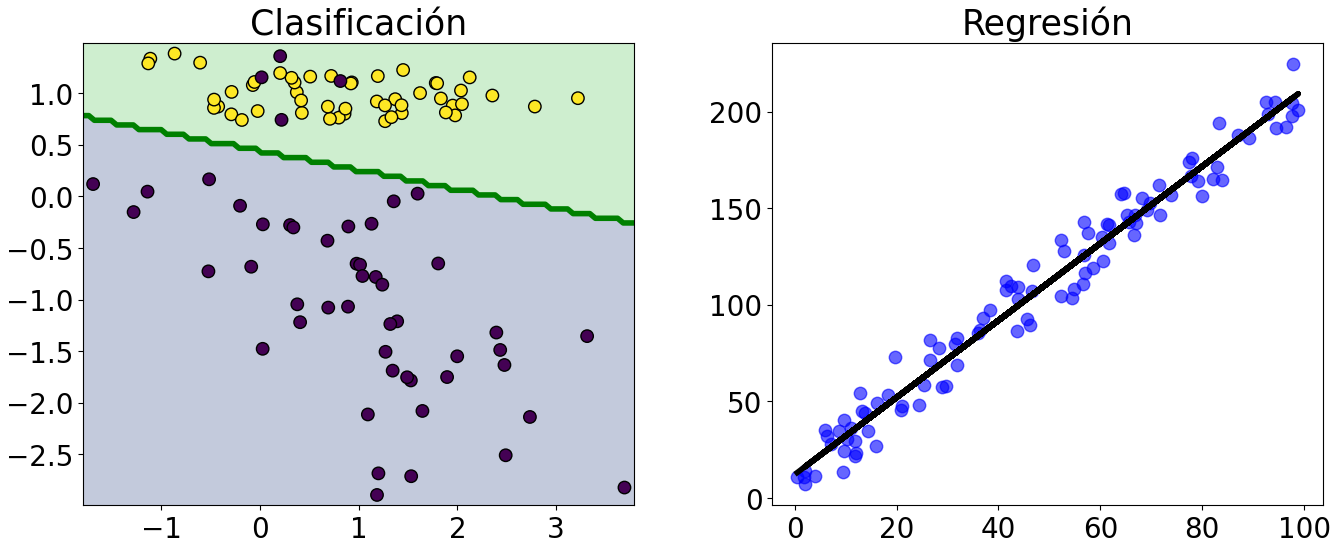
\includegraphics[width=0.8\linewidth]{img/clasi-regresion.png}
    \caption[Ejemplos de problemas de clasificación y regresión.]{Ejemplos de problemas de clasificación y regresión. A la izquierda, se muestra un problema de clasificación binario, donde se busca encontrar el hiperplano (línea verde) que separe ambos conjuntos de datos etiquetados. A la derecha, se muestra un problema de regresión, donde se busca encontrar la mejor aproximación (línea negra) al conjunto de datos. Imagen original del autor.}\label{fig:clasi-regresion}
\end{figure}

Dentro del marco del aprendizaje supervisado, donde el principal objetivo del modelo es aprender a predecir la salida correcta para nuevos ejemplos no conocidos, basándose en las relaciones y patrones extraídos al trabajar con los datos etiquetados, podemos dividir los problemas en dos categorías principales: problemas de clasificación en los que se asigna una salida o clase (discreta) a cada entrada y problemas de regresión en los que se predice un valor continuo para cada entrada (véase~\autoref{fig:clasi-regresion}). De cara al desarrollo de nuestro trabajo, abordaremos ambos tipos de problemas. En particular, en los problemas de clasificación nos centraremos en la clasificación de imágenes.\newline

El aprendizaje profundo o \emph{deep learning} (DL) (\cite{Bishop2023},~\cite{Prince2023} y~\cite{LeCun2015}) representa un área del aprendizaje automático que utiliza redes neuronales artificiales, inspiradas en la estructura y función del cerebro humano, con múltiples capas, conocidas como redes neuronales profundas (\cite{Goodfellow2016} y~\cite{Schmidhuber2015}), con el propósito de identificar y modelar patrones complejos y extraer representaciones jerárquicas en grandes volúmenes de datos.\newline

\section{Redes neuronales artificiales}\label{sec:redes-neuronales-artificiales}

Una red neuronal artificial o \emph{artificial neural network} (ANN) (\cite{Bishop1995},~\cite{Ripley1996}) es un modelo de aprendizaje automático que toma decisiones de manera similar al funcionamiento del cerebro humano, a partir de las interconexiones que presentan las neuronas biológicas, que se organizan en diferentes capas interconectadas. Estas conexiones simulan las interacciones entre las neuronas biológicas, permitiendo que la red procese información y aprenda de manera similar al propio cerebro humano.\newline

De manera similar al cerebro humano, una red neuronal artificial está formada por neuronas artificiales (véase~\autoref{fig:neuronasbioyartificial}), también llamadas unidades. Estas unidades se agrupan en diferentes capas formando la arquitectura global de la red neuronal. Cada capa puede contener un número variable de unidades, lo que permite adaptar la red a la complejidad del problema a resolver.\newline

\begin{figure}[h]
    \centering
    \subfloat{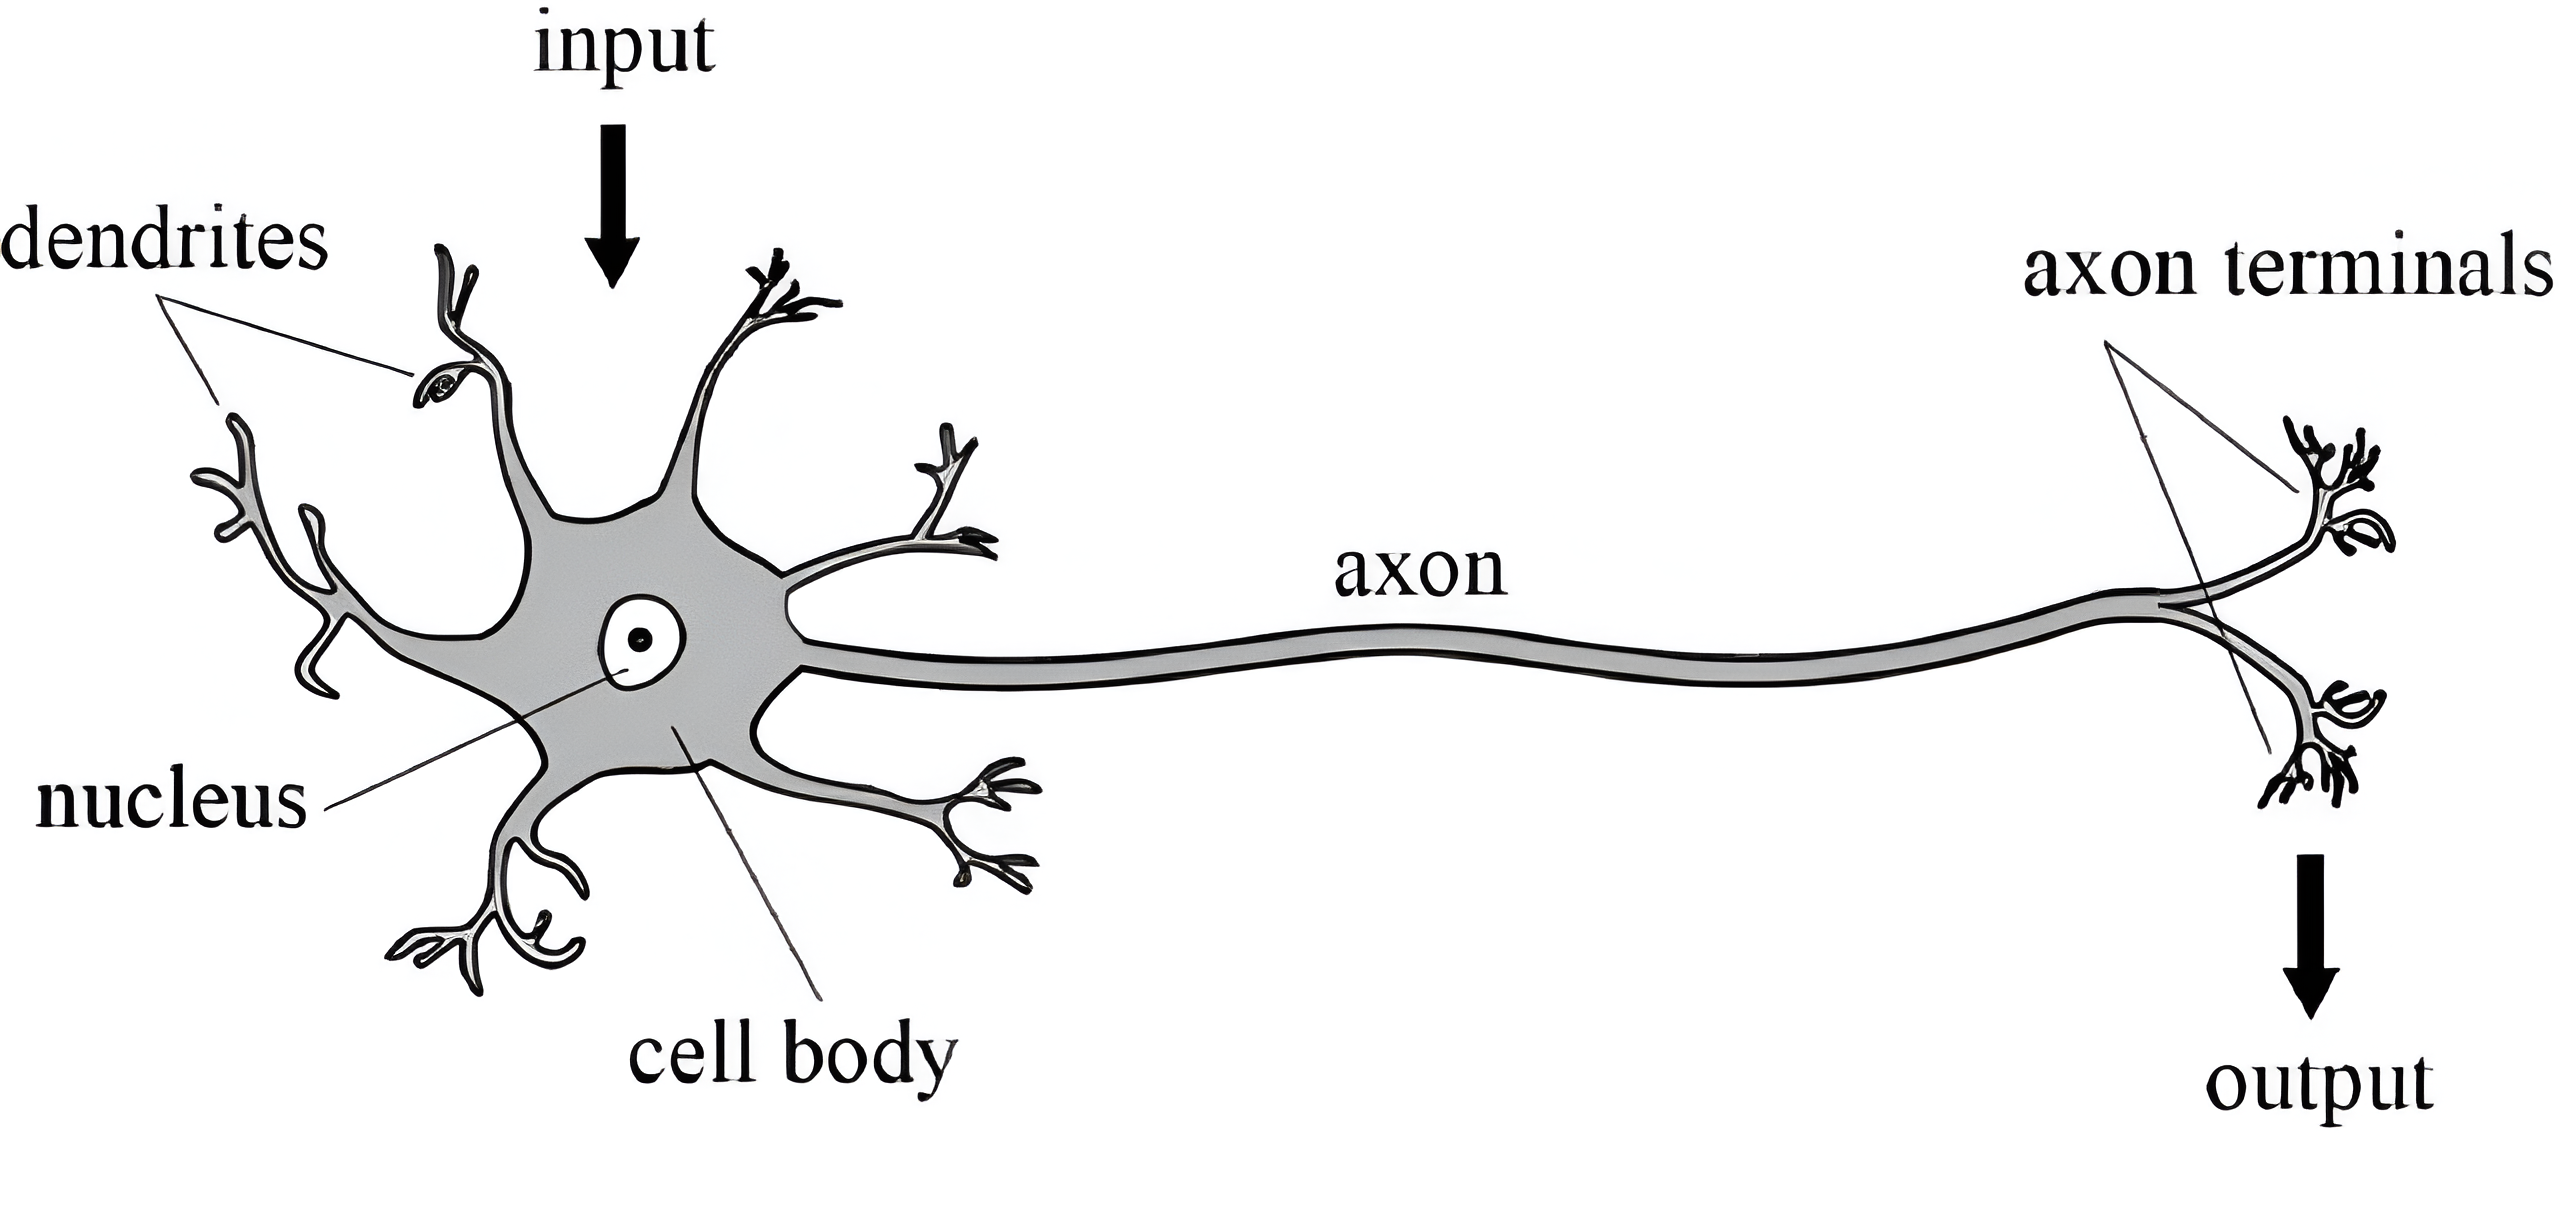
\includegraphics[width=0.45\textwidth]{img/biological-neuron.png}}
    \hfill
    \subfloat{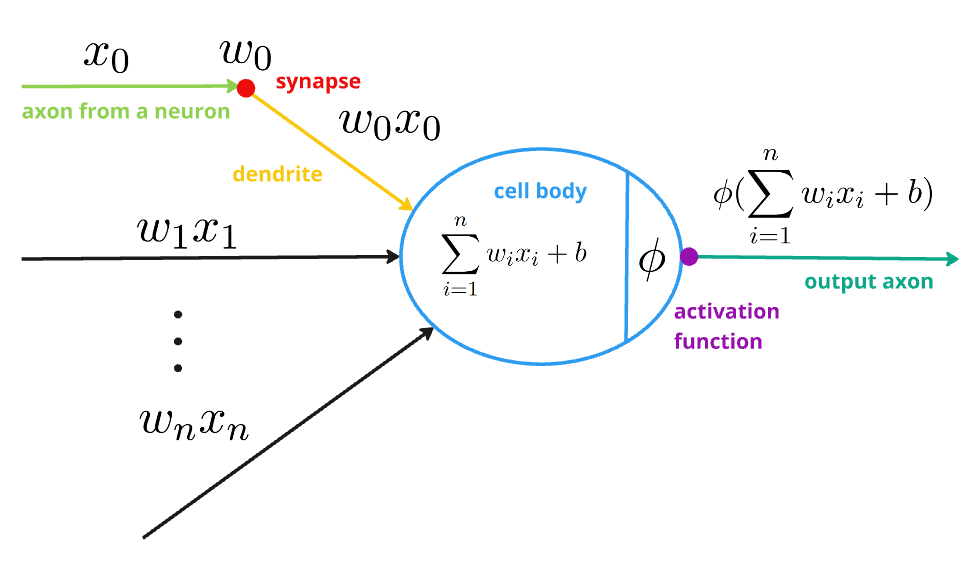
\includegraphics[width=0.45\textwidth]{img/artificial-neuron.png}}
    \caption[Ejemplos de neurona biológica~\cite{Neves2018} y neurona artificial (basada en~\cite{Li2024}).]{Ejemplos de una neurona biológica~\cite{Neves2018} (izquierda) y una neurona artificial (derecha) basada en~\cite{Li2024}.}\label{fig:neuronasbioyartificial}
\end{figure}

A alto nivel, el funcionamiento de una red neuronal artificial se divide en, al menos, tres capas principales, constituidas por una capa de entrada, una capa oculta y una capa de salida. En la primera capa o capa de entrada, la información del mundo exterior entra en la red neuronal. Dicha información es procesada y propagada al resto de capas mediante un proceso conocido como propagación hacia delante o \emph{forward propagation}, permitiendo que la información fluya desde la capa de entrada hacia las capas sucesivas.\newline

En la capa oculta o capa de procesamiento, las unidades reciben las salidas de la capa anterior y se encargan de procesar la información mediante conexiones ponderadas (llamadas pesos) y funciones de activación (encargadas de introducir no linealidad en el modelo, permitiendo que la red aprenda y represente relaciones complejas entre las entradas y las salidas), extrayendo características y patrones relevantes de los datos. Los pesos obtenidos controlan la influencia que cada neurona de la capa anterior tiene sobre la neurona actual. Las redes neuronales artificiales pueden tener una gran cantidad de capas ocultas, lo que permite un procesamiento más profundo y detallado de la información. Cada capa oculta analiza la salida de la capa anterior, la procesa aún más y la pasa a la siguiente capa, de modo que, a medida que se avanza por la red, se generan representaciones internas cada vez más abstractas de la entrada original.\newline

Finalmente, en la última capa o capa de salida, la red produce el resultado final en función del problema que se trate y de la predicción calculada haciendo uso de los pesos ajustados en las capas ocultas. La naturaleza de la salida varía según el tipo de tarea que se realice: en un problema de clasificación, la salida es un valor discreto que indica la clase a la que pertenece la entrada, mientras que en un problema de regresión, la salida es un valor continuo que representa una predicción numérica. Por tanto, esta capa es la que traduce la información procesada por la red en un resultado interpretable y acorde con el objetivo del problema.\newline

Por tanto, el proceso de entrenamiento de una red neuronal artificial es un proceso iterativo en el que la red ajusta sus pesos para aprender a realizar tareas específicas. Para llevar a cabo este proceso, es fundamental un conjunto de datos o ejemplos de entrenamiento que sea lo suficientemente representativo, ya que de este conjunto se extraerán los patrones relevantes que la red necesitará aprender.\newline

\subsection{Redes neuronales convolucionales}\label{subsec:redes-neuronales-convolucionales}

Las redes neuronales convolucionales o \emph{convolutional neural networks} (CNN) (\cite{LeCun1989}, \cite{LeCun1998}) son un tipo especial de red neuronal artificial que se utiliza principalmente en procesamiento de imágenes, reconocimiento visual y tareas relacionadas con datos que tienen una estructura de rejilla (matriz multidimensional), como imágenes, vídeos o señales de audio. Una de las características más destacadas de las redes neuronales convolucionales es su capacidad para realizar la extracción automática y jerárquica de características de los datos de entrada, lo que las hace especialmente poderosas para tareas que requieren reconocer patrones complejos en los datos.\newline

Esta capacidad de aprendizaje jerárquico de características es una de las principales razones por las que las CNN son tan eficaces, ya que permiten a la red identificar patrones relevantes sin necesidad de intervención humana para diseñar características específicas, lo que las vuelve especialmente interesantes en áreas como la visión por computador, donde han impulsado avances significativos en aplicaciones como el reconocimiento de imágenes, la segmentación semántica y la detección de objetos, entre otras.\newline

Las redes neuronales convolucionales incluyen varias capas especializadas que las distinguen de las redes neuronales artificiales tradicionales: las capas de convolución, encargadas de la extracción de características de la entrada; las capas de agrupación o \emph{pooling}, responsables de la reducción de la dimensionalidad de la entrada sin perder las características importantes y las capas totalmente conectadas o \emph{fully connected}, que se encuentran en la parte final de la red y que permiten combinar de manera efectiva las características extraídas por las capas anteriores para realizar la predicción final (véase~\autoref{fig:cnn}). Estas capas operan de manera conjunta, transformando la entrada y extrayendo progresivamente las características más relevantes, las cuales se van refinando y volviéndose más abstractas conforme se avanza por la red.\newline

\begin{figure}[h]
    \centering
    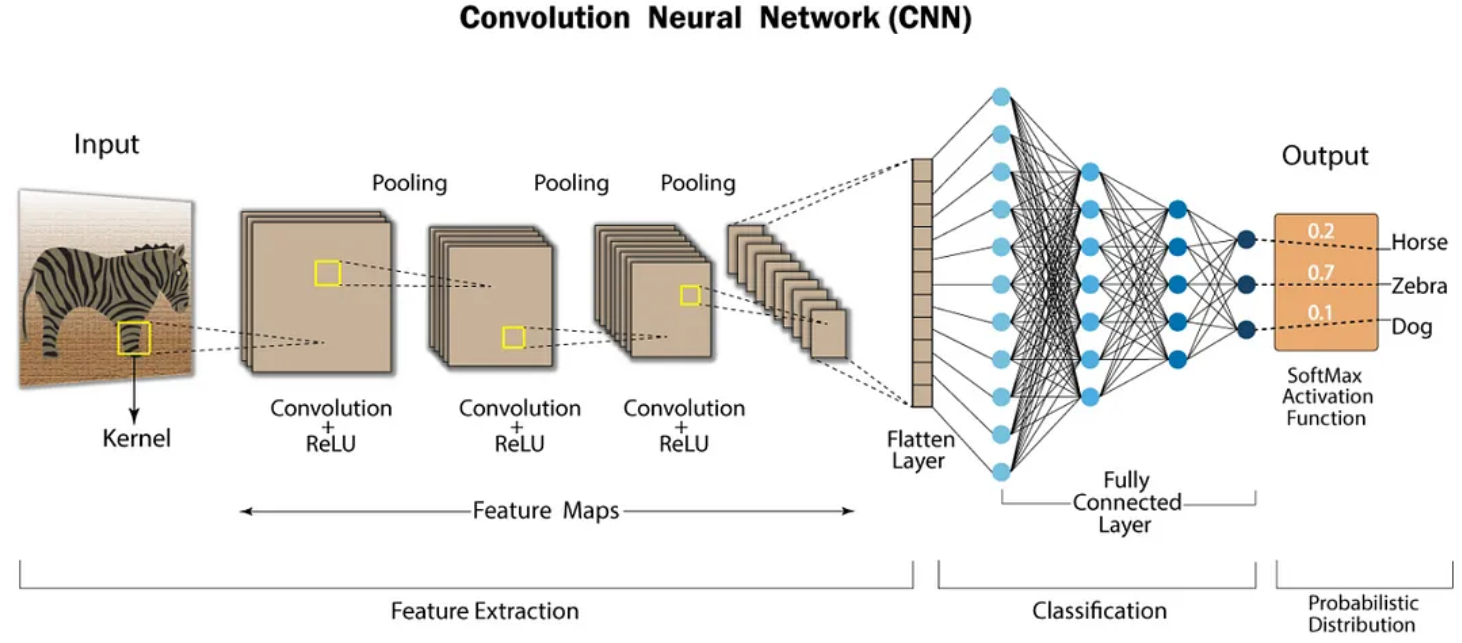
\includegraphics[width=0.8\linewidth]{img/cnn.png}
    \caption[Ejemplo de CNN utilizada para clasificación de imágenes~\cite{CNNSwapna}.]{Ejemplo de CNN utilizada para clasificación de imágenes~\cite{CNNSwapna}. La entrada a la red es una imagen en formato RGB. La extracción de características se realiza mediante varias capas convolucionales, seguidas de funciones de activación y capas de pooling, las cuales ayudan a reducir la dimensionalidad. Posteriormente, las características extraídas se aplanan (\textit{flattening}) y se envían a las capas totalmente conectadas. Finalmente, la salida pasa por una función de activación, en este caso softmax, que genera una distribución de probabilidad sobre las posibles clases de salida.}\label{fig:cnn}
\end{figure}

A continuación se describen las principales capas que conforman una red neuronal convolucional. Se incluyen tanto las capas exclusivas de este tipo de red como aquellas que comparte con las redes neuronales tradicionales:


\subsubsection{Capa de convolución}

La capa convolucional es un componente fundamental y exclusivo de las CNN, diseñada para extraer características locales de datos estructurados en forma de matrices multidimensionales. Su funcionamiento se basa en utilizar matrices de valores, conocidas como filtros o \emph{kernels}, que se deslizan sobre la entrada aplicando la operación matemática de convolución.\newline

La convolución es una operación lineal que consiste en desplazar un filtro sobre la entrada, realizando en cada posición una multiplicación elemento a elemento entre los valores del filtro y los de la entrada (diferente de una multiplicación matricial convencional). Posteriormente, se suman estos productos para obtener un único valor de salida. Este proceso se repite hasta deslizar el filtro a lo largo de toda la entrada, obteniendo una nueva matriz denominada mapa de características.\newline

Los valores de los filtros actúan como los pesos que la propia red aprende y optimiza de forma iterativa para maximizar la extracción de características relevantes de la entrada. Además, el número de filtros aplicados sobre cada entrada influye directamente en el mapa de características de salida resultante. Así, a mayor cantidad de filtros, la profundidad del mapa de características resultantes también es mayor.\newline

\begin{figure}[h]
    \centering
    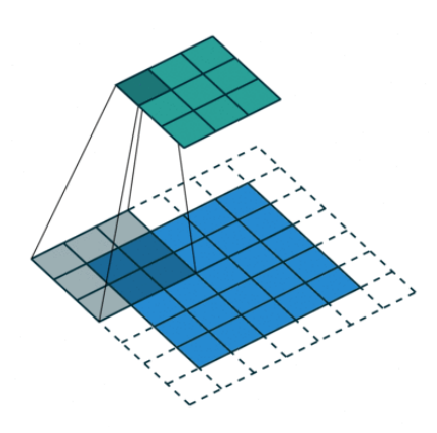
\includegraphics[width=0.5\linewidth]{img/convolucion.png}
    \caption[Ejemplo de convolución con padding~\cite{Saha2018}.]{Ejemplo de convolución con padding~\cite{Saha2018}. El color azul hace referencia a la entrada, mientras que el color verde denota el resultado de la convolución. En particular, el color verde oscuro destaca el resultado de la convolución que se realiza sobre la zona grisácea de la imagen, utilizando, en este caso, un filtro de tamaño 3x3. Por otra parte, las cuadrículas punteadas hacen referencia al padding agregado.}\label{fig:convolucion}
\end{figure}

Como se puede observar en la~\autoref{fig:convolucion}, la propia naturaleza de la operación de convolución modifica la dimensionalidad de la entrada. Sin embargo, esto no siempre es deseable, ya que en determinadas ocasiones preferiremos mantener la dimensión original de la entrada. Para solucionar este problema, se introduce el concepto de relleno o \emph{padding}, consistente en agregar información adicional alrededor de la entrada, con el fin de preservar su dimensionalidad.\newline

Por otra parte, la elección de la siguiente zona sobre la que se realizará la convolución viene determinada por el tamaño de paso o \emph{stride}. Generalmente, se utiliza un stride de $1$, lo que significa que desplazamos el filtro de manera adyacente una posición en cada paso. Sin embargo, también es posible reducir la dimensionalidad de la entrada modificando el stride, como puede observarse en la~\autoref{fig:convolucion}, donde, a pesar de utilizar un relleno de una posición para mantener la dimensionalidad, el tamaño del mapa de activación resultante es inferior al tamaño original de la entrada, pues se está utilizando un stride de 2.\newline

En conlusión, el objetivo principal de la capa de convolución es extraer características relevantes de la entrada. Para ello, se utilizan filtros cuyos pesos son aprendidos y optimizados por la propia red. En las primeras capas convolucionales, dado que el tamaño de la entrada es mayor, se detectan principalmente características de bajo nivel, como bordes y texturas. A medida que la información avanza por la red, las capas posteriores capturan patrones más complejos y abstractos. De este modo, mediante la combinación de múltiples capas convolucionales, la red logra desarrollar una representación jerárquica de la entrada.\newline

\subsubsection{Capa de pooling}

Las capas de pooling son otro componente esencial y exclusivo en las redes neuronales convolucionales, ya que su función principal es reducir la dimensionalidad de las representaciones producidas por las capas de convolución, simplificando los mapas de características mientras se preservan las características más relevantes, lo que conlleva una reducción en la cantidad de parámetros y en la complejidad computacional de la red.\newline

El pooling es una operación que toma un conjunto de valores de un mapa de características y lo reduce a un solo valor, con el propósito de submuestrear la información, introduciendo cierta invarianza espacial frente a pequeñas variaciones espaciales de la entrada, lo que permite detectar patrones aunque se encuentren ligeramente desplazados en la imagen, aumentando la robustez de la red.\newline

El tipo de pooling más comúnmente utilizado es el denominado \emph{max pooling} (véase~\autoref{fig:convolucion}), que selecciona el valor máximo de un conjunto de valores dentro de una región del mapa de características. Otras alternativas incluyen el \emph{average pooling}, que selecciona el valor promedio del conjunto de valores de la región del mapa de características utilizada y el \emph{global pooling}, que reduce el mapa de características a un único valor. En nuestro proyecto se hará uso del max pooling, integrado en algunas de las arquitecturas que utilizamos para los experimentos.\newline

\begin{figure}[h]
    \centering
    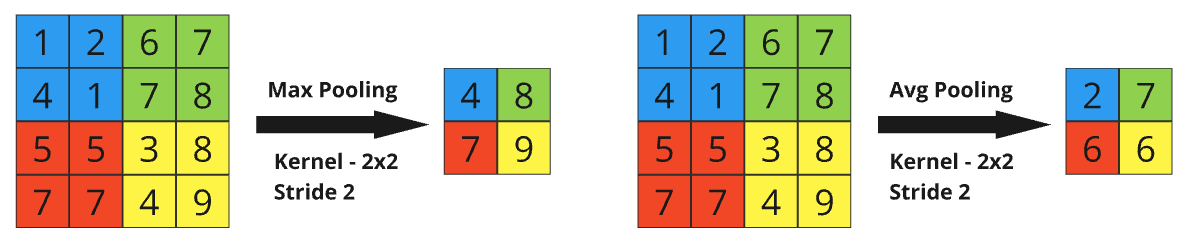
\includegraphics[width=0.8\linewidth]{img/pooling.png}
    \caption[Ejemplos de pooling utilizados en CNN.]{Ejemplos de pooling utilizados en CNN. A la izquierda, se muestra el max pooling, donde se selecciona el valor máximo de una determinada región (en este caso 2x2). A la derecha, se muestra el average pooling, donde se selecciona el valor promedio de la región influida por el filtro. Imagen original del autor.}\label{fig:pooling}
\end{figure}

\subsubsection{Capa totalmente conectada}

Las capas totalmente conectadas o densas (\emph{fully connected}) son un componente fundamental en las redes neuronales, presentes tanto en las tradicionales, formando la arquitectura básica de una ANN, como en las redes convolucionales. Estas capas se encuentran normalmente en las etapas finales de la red, encargándose de realizar la interpretación final de las características extraídas por las capas anteriores (véase~\autoref{fig:cnn}).\newline

Antes de entrar a una capa densa, la salida de las capas anteriores debe aplanarse (\emph{flattening}) en un vector unidimensional puesto que, generalmente, la salida de las capas anteriores tendrán forma matricial o tensorial, lo que impide que puedan ser procesadas directamente por las capas densas. De esta manera, el número de unidades de la primera capa densa se corresponde con el número de componentes del vector unidimensional.\newline

Estas capas combinan y procesan las características extraídas de las capas anteriores y tienen la posibilidad de capturar relaciones globales al conectar cada unidad de una capa con todas las unidades de la siguiente capa por medio de conexiones con pesos entrenables, lo que produce que la mayor parte de los pesos entrenables de una red suelan concentrarse en estas capas debido al elevado número de conexiones que presentan.\newline

\subsubsection{Capa de activación}\label{subsubsec:capa-de-activacion}

Las capas o funciones de activación son las responsables de introducir no linealidad en el modelo, transformando la combinación lineal de las entradas mediante una función matemática. Esta transformación es esencial para que la red pueda aprender y representar patrones complejos en los datos.\newline

Sin funciones de activación, una red neuronal se reduciría simplemente a una combinación lineal de las entradas, sin importar cuántas capas tuviera. Incluso si solo se usaran funciones de activación lineal, la red neuronal se comportaría como una función lineal. Como menciona Bishop en su libro: ``Si se considera que las funciones de activación de todas las unidades ocultas de una red son lineales, entonces para cualquier red de este tipo siempre podemos encontrar una red equivalente sin unidades ocultas'' (\cite{Bishop2006}), limitando la capacidad de la red para modelar relaciones complejas.\newline

Por tanto, las capas de activación se colocan después de cada capa lineal (como las capas convolucionales o las capas densas) en una red neuronal, con el objetivo de permitir que dicha capa pueda aprender también relaciones no lineales. A lo largo de este trabajo, se utilizarán algunas de las funciones de activación más comunes y ampliamente empleadas en el campo del aprendizaje profundo, entre las que se incluyen:

\begin{itemize}
    \item \textbf{ReLU (Rectified Linear Unit)}: Es una de las funciones de activación más utilizadas, especialmente en las capas ocultas de las redes neuronales profundas, debido a su simplicidad computacional, lo que permite acelerar el proceso de entrenamiento. Su expresión matemática es la siguiente
    
    \[
        \text{ReLU}(x) = \max(0, x)
    \]

    donde $x$ representa la entrada a la función, que corresponde con la salida lineal de la capa anterior de la red neuronal. Sin embargo, esta función de activación puede provocar el problema de ``neuronas muertas'', donde algunas unidades dejan de activarse permanentemente, cuando su entrada es negativa o $0$ (véase~\autoref{fig:funcionesactivacion}).

    \item \textbf{Softmax:} Se utiliza principalmente en la capa de salida para tareas de clasificación multiclase. Convierte un vector de valores reales en un vector de probabilidades que suman $1$, facilitando la interpretación de las salidas como probabilidades de pertenencia a cada clase. Su expresión matemática es la siguiente
 
    \[
        \text{Softmax}(x_i) = \frac{e^{x_i}}{\sum_{j=1}^{K} e^{x_j}}
    \]

    donde $x_i$ representa la entrada correspondiente a la clase $i$-ésima antes de aplicar la activación y $K$ el número de clases. Esta función de activación es una generalización de la función sigmoide para clasificación multiclase. Por tanto, para el caso de $K=2$ (clasificación binaria), esta función se reduce a la función sigmoide.\newline

\end{itemize}

\begin{figure}[h]
    \centering
    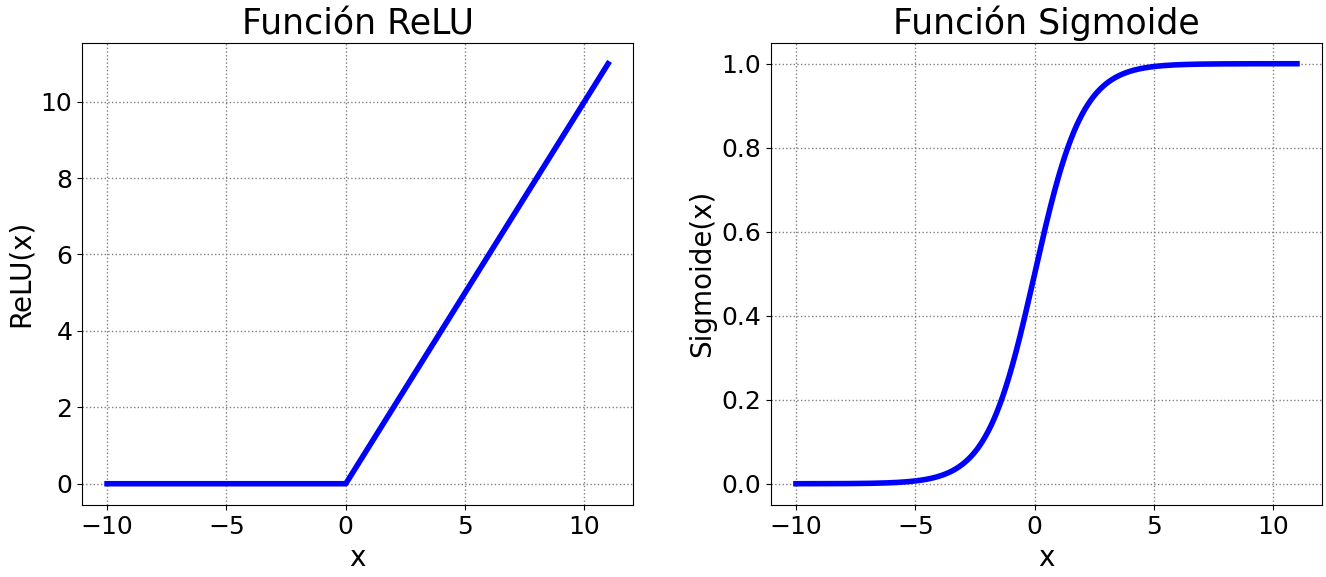
\includegraphics[width=0.8\linewidth]{img/funcionesactivacion.png}
    \caption[Ejemplos de funciones de activación utilizadas en CNN.]{Ejemplos de funciones de activación utilizadas en CNN. A la izquierda, se muestra la función ReLU, donde se observa como deja invariante los valores positivos, estableciendo a cero los valores negativos. A la derecha, se muestra la función sigmoide, que mapea los valores de entrada a un rango entre $0$ y $1$. Imagen original del autor.}\label{fig:funcionesactivacion}
\end{figure}

\chapter{El dilema clásico del aprendizaje}\label{ch:dilema-aprendizaje}

En este capítulo, como preámbulo antes de adentrarnos en el \textit{Deep Double Descent}, presentaremos algunos conceptos básicos de la sabiduría clásica del aprendizaje automático que nos harán entender de manera más precisa el suceso. Las fuentes principales utilizadas a lo largo de este capítulo son extractos de~\cite{Mostafa2012, Bishop2006}.\newline

\section{Concepto de aprendizaje}\label{sec:concepto-de-aprendizaje}
El aprendizaje, dentro del marco del aprendizaje automático, puede considerarse como un proceso en el que se busca encontrar una función $g$ que aproxime lo máximo posible a la función objetivo $f$, que describe las relaciones y patrones subyacentes entre las entradas y salidas de los datos. Dado que la función objetivo es siempre desconocida, pues, en otro caso, no habría que aprender nada al conocer directamente la función objetivo, serán los propios datos etiquetados los que nos ayuden, mediante el entrenamiento de modelos, a obtener una función aproximadora de dicha función objetivo.\newline

En nuestro caso, de cara a trabajar con el aprendizaje supervisado, consideraremos los siguientes componentes del mismo:
\begin{itemize}
    \item Espacio muestral $\mathcal{X}$: representa el conjunto de todas las posibles entradas $x$ que el modelo puede recibir, tomadas de manera independiente siguiendo alguna (sin restricción) distribución de probabilidad $P$ en $\mathcal{X}$.
    \item Conjunto $\mathcal{Y}$: compuesto por todas las posibles salidas (etiquetas) que el modelo debe predecir.
    \item Función objetivo $f: \mathcal{X} \rightarrow \mathcal{Y}$, que representa la función objetivo y desconocida que asigna cada entrada $x \in \mathcal{X}$ a una salida $y \in \mathcal{Y}$.
    \item Un conjunto de datos de entrenamiento $\mathcal{D}$, formado por pares $(x, y)$ con $x \in \mathcal{X}$ y $y \in \mathcal{Y}$, donde $f(x) = y$.
    \item Un conjunto de hipótesis $\mathcal{H}$, donde se encontrarán todas las funciones candidatas que el modelo puede aprender para aproximar la función objetivo. Es decir, $\mathcal{H} = \{h: X \rightarrow Y / X \subseteq \mathcal{X}, Y \subseteq \mathcal{Y}\}$. 
    \item Un algoritmo de aprendizaje $\mathcal{A}$, que es el encargado de elegir una función candidata $h \in \mathcal{H}$ que aproxime a la función objetivo $f$.\newline
\end{itemize}

De este modo, el modelo de aprendizaje automático, por medio del algoritmo de aprendizaje, será el encargado de seleccionar la función candidata $g \in \mathcal{H}$ que mejor aproxime a la función objetivo $f$ utilizando el conjunto de datos de entrenamiento disponible, con el propósito de que la función candidata $g$ siga replicando a la función objetivo $f$ ante nuevos datos no disponibles.\newline

\begin{figure}[h]
    \centering
    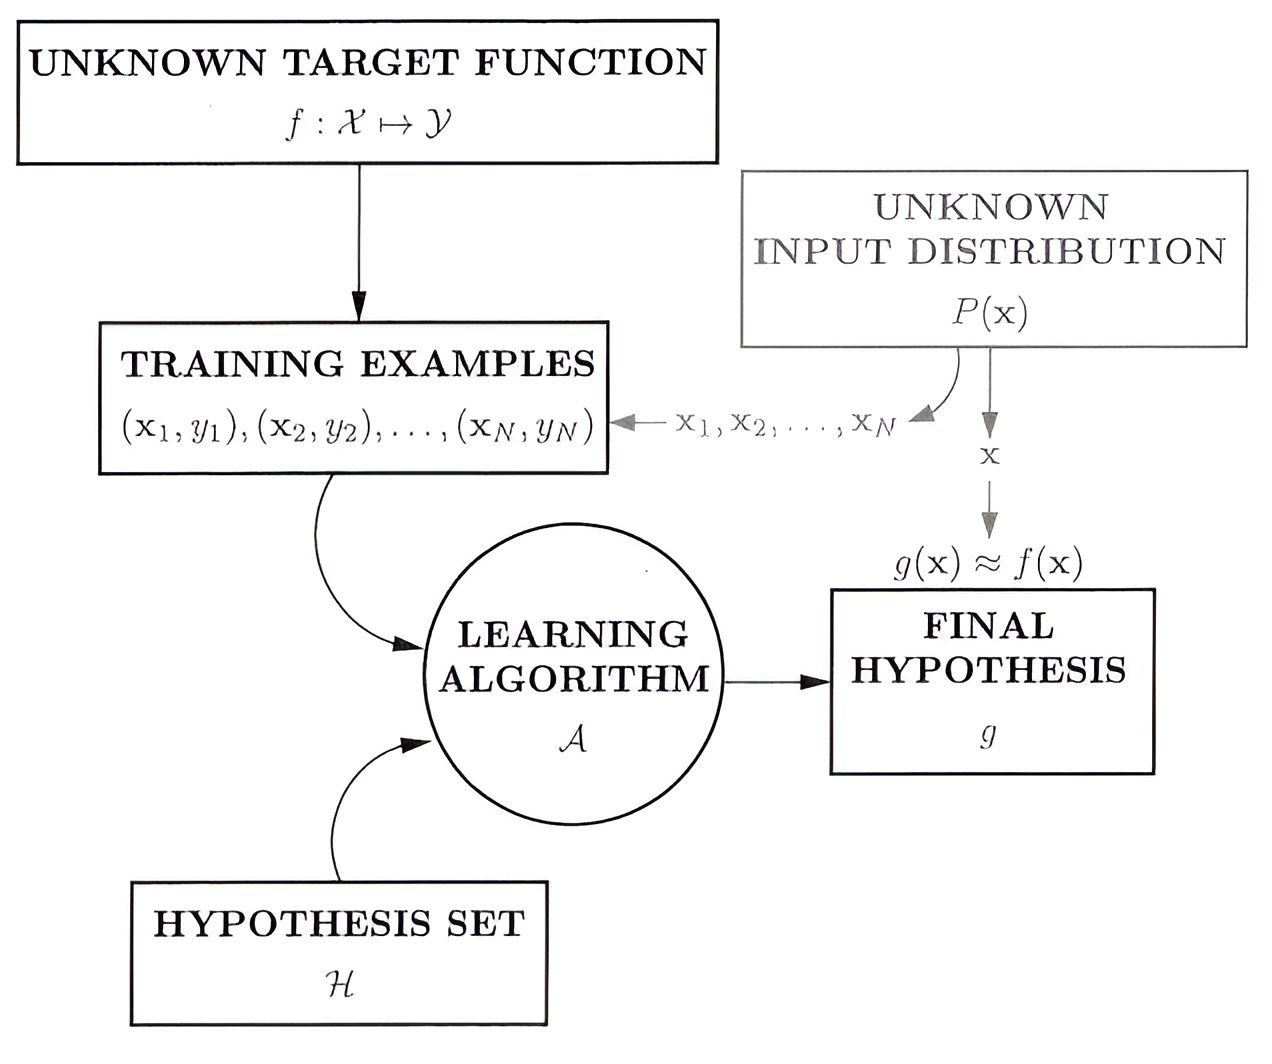
\includegraphics[width=0.7\linewidth]{img/learning-diagram.png}
    \caption[Diagrama representando el concepto básico de aprendizaje.]{Diagrama representando el concepto básico de aprendizaje~\cite{Mostafa2012}. El algoritmo de aprendizaje (\textit{learning algorithm}), utilizando los ejemplos de entrenamiento (\textit{training examples}) muestreados de una distribución de probabilidad desconocida (\textit{unknown input distribution}), buscará en el conjunto de hipótesis (\textit{hypothesis set}) la mejor aproximación (\textit{final hypothesis}) a la función objetivo desconocida (\textit{unknown target function}) que se desea aprender.}\label{fig:learning-diagram}
\end{figure}

\subsection{Descenso de gradiente y aprendizaje}\label{subsec:descenso-gradiente}

El descenso de gradiente o \emph{gradient descent} (GD) es la columna vertebral del aprendizaje en redes neuronales y, en general, sienta las bases para las técnicas de aprendizaje automático y aprendizaje profundo. Se trata de un algoritmo de optimización sin restricciones cuyo objetivo principal es minimizar la función de pérdida o error del modelo. Dicha función de pérdida mide cuán lejos están las predicciones realizadas por el modelo de los valores reales, y minimizarla conllevará asociada una mejora en la precisión y capacidad de generalización del modelo.\newline

La idea subyacente del descenso de gradiente se basa en calcular de forma iterativa el gradiente, es decir, la derivada parcial de la función de pérdida con respecto a los parámetros. A partir de este gradiente, nos desplazamos en la dirección opuesta al mismo (véase Ecuación~\eqref{eq:descenso-gradiente}), ya que esta zona indica la dirección del descenso más pronunciado en la función de pérdida. De este modo, se garantiza que los parámetros se ajusten para minimizar progresivamente la pérdida, mejorando así el rendimiento del modelo.\newline

A continuación se muestra la expresión del descenso de gradiente:

\begin{equation}
    \mathbf{w}^{(\tau + 1)} = \mathbf{w}^{(\tau)} - \eta \nabla E(\mathbf{w}^{(\tau)})
    \label{eq:descenso-gradiente}
\end{equation}

donde $\mathbf{w}^{(\tau + 1)}$ representa los valores de los parámetros actualizados, $\mathbf{w}^{(\tau)}$ representa los valores de los parámetros antes de la actualización, $\eta$ es un hiperparámetro, denominado tasa de aprendizaje o \emph{learning rate}, que controla el tamaño del paso en cada actualización y $\nabla E(\mathbf{w}^{(\tau)})$ indica el gradiente de la función de pérdida con respecto a los parámetros, es decir, la dirección y magnitud en la que la función de pérdida aumenta de manera más rápida.\newline

Es importante destacar que la tasa de aprendizaje ($\eta$) desempeña un papel esencial en el proceso de optimización. Si se elige un valor demasiado pequeño de la misma, el modelo podría tardar mucho en converger (véase~\autoref{fig:gradientdescent}), requiriendo un número elevado de épocas o iteraciones para alcanzar un mínimo adecuado de la función de pérdida. Por el contrario, si se selecciona un valor demasiado grande, el modelo podría no converger e incluso divergir, oscilando alrededor del mínimo sin lograr estabilizarse o incluso aumentando la pérdida. Es por esto que, la mejor estrategia suele consistir en utilizar un valor grande al inicio del entrenamiento, para acelerar el entrenamiento, y reducirlo progresivamente a medida que avanza, con el objetivo de no divergir y estabilizarnos en el mínimo.\newline

\begin{figure}[h]
    \centering
    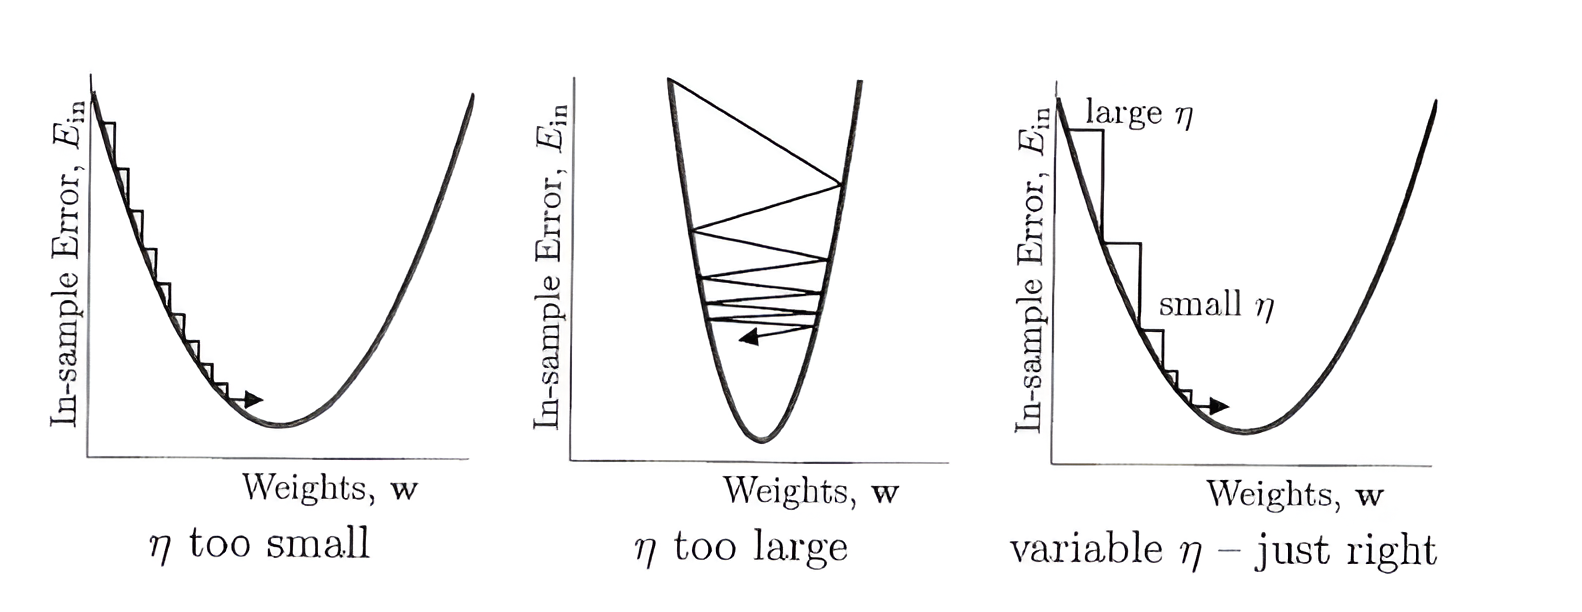
\includegraphics[width=0.9\linewidth]{img/gradientdescent.png}
    \caption[Distintas tasas de aprendizaje para el descenso de gradiente~\cite{Mostafa2012}.]{Distintas tasas de aprendizaje para el descenso de gradiente~\cite{Mostafa2012}. En la primera imagen, una tasa de aprendizaje pequeña lleva a una convergencia lenta con muchas actualizaciones. En la imagen central, una tasa demasiado grande provoca saltos bruscos que pueden impedir la convergencia. En la última imagen, una tasa variable comienza con un valor grande para avanzar rápido y disminuye progresivamente, logrando una convergencia rápida y estable.}\label{fig:gradientdescent}
\end{figure}

Asimismo, existen variantes del descenso de gradiente, como el descenso de gradiente estocástico (SGD), que actualiza los parámetros utilizando cada ejemplo de entrenamiento, lo que provoca que sea muy lento cuando trabajamos con grandes volúmenes de datos. Por otro lado, nos encontramos el descenso de gradiente por lotes (Batch Gradient Descent), que utiliza el conjunto completo de datos de entrenamiento para calcular el gradiente y actualizar los parámetros, lo que permite realizar una convergencia más estable y precisa. Sin embargo, suele ser más costoso tanto computacionalmente como en términos de tiempo. Es por esto que, en el desarrollo de este proyecto, se utilizará el descenso de gradiente por mini-lotes (Mini-batch Gradient Descent), que combina lo mejor de ambos métodos, ya que utiliza subconjuntos de datos de entrenamiento para realizar la actualización de parámetros.\newline

En resumen, el descenso de gradiente permite que la red neuronal mejore sus predicciones a lo largo de múltiples iteraciones o épocas. Cada vez que el modelo procesa un conjunto de datos, calcula el error y ajusta sus parámetros para aprender de los errores cometidos, repitiéndose este proceso hasta que la función de pérdida alcanza un valor mínimo aceptable.\newline

\subsubsection{Optimizador Adam}\label{subsubsec:optimizador-adam}
De cara al interés de nuestro proyecto, trabajaremos con el optimizador \textbf{Adam} (\textit{Adaptive Moment Estimation},~\cite{Diederik2017}). Este optimizador se basa en las ideas de los algoritmos \textbf{Momentum} y \textbf{RMSProp}, combinando sus principales ventajas para lograr una convergencia más rápida y estable durante el entrenamiento de modelos de aprendizaje profundo.\newline

El método de \textit{Momentum} mejora al SGD acumulando un promedio móvil de los gradientes pasados. La actualización de los parámetros se realiza de la siguiente forma:

\[
    \begin{aligned}
        m_{\tau} &= \beta_1 \cdot m_{\tau-1} + (1 - \beta) \cdot \nabla E(w_{\tau - 1}), \\
        w_{\tau} &= w_{\tau - 1} - \eta \cdot m_\tau
    \end{aligned}
\]

donde el término $\beta$ actúa como un factor de decaimiento que regula la influencia de los gradientes anteriores en la actualización actual. Por su parte, $\eta$ representa la tasa de aprendizaje. Así, la variable $m_{\tau}$ corresponde al promedio móvil de los gradientes, es decir, una estimación de primer orden que suaviza la dirección de la actualización.\newline

El algoritmo \textit{RMSProp} adapta la tasa de aprendizaje en función de la magnitud reciente de los gradientes. Para lograrlo, calcula un promedio móvil de los cuadrados de los gradientes, lo que permite ajustar dinámicamente la escala de la actualización para cada parámetro:

\[
    \begin{aligned}
        v_{\tau} &= \beta \cdot v_{\tau-1} + (1- \beta)(\nabla E(w_{\tau-1})), \\
        w_{\tau} &= w_{\tau-1} - \eta \cdot \frac{\nabla E(w_{\tau-1})}{\sqrt{v_{\tau}}+\epsilon},
    \end{aligned}
\]

donde el factor $\beta$ actúa, al igual que en el caso de Momentum, como un factor de olvido que determina cuánto influyen los valores anteriores en la media móvil. Así, $v_{\tau}$ representa una estimación de segundo orden, correspondiente al promedio móvil de los cuadrados de los gradientes. Además, el término $\epsilon$ se introduce para mejorar la estabilidad numérica, evitando divisiones por cero durante la actualización de los parámetros.\newline

Finalmente, \textit{Adam} combina los enfoques anteriores, manteniendo simultáneamente estimaciones de primer y segundo orden. Las actualizaciones se realizan de la siguiente manera:

\begin{equation}
    \begin{aligned}
        m_{\tau} &= \beta_1 \cdot m_{\tau-1} + (1 - \beta_1) \cdot \nabla E(w_{\tau - 1}), \\
        v_{\tau} &= \beta_2 \cdot v_{\tau-1} + (1 - \beta_2) \cdot \nabla E(w_{\tau - 1}).
    \end{aligned}
\end{equation}

Dado que $m_\tau$ y $v_\tau$ están inicializados en cero, Adam introduce una corrección de sesgo:

\begin{equation}
    \begin{aligned}
        \hat{m_\tau} = \frac{m_\tau}{1- \beta_1^{\tau}}, \\
        \hat{v_\tau} = \frac{v_\tau}{1- \beta_2^{\tau}}.
    \end{aligned}
\end{equation}

Como paso final, los parámetros se actualizan de la siguiente forma:

\begin{equation}
    w_{\tau} = w_{\tau - 1} - \frac{\eta}{\sqrt{\hat{v}_{\tau}} + \epsilon} \cdot \hat{m}_{\tau}.
\end{equation}

Este enfoque combina la dirección promedio de los gradientes con una tasa de aprendizaje adaptativa. Por un lado, acumular gradientes pasados permite suavizar la trayectoria y evitar oscilaciones y por otro, normalizar mediante una estimación de segundo orden ajusta la tasa de aprendizaje de manera dinámica para cada parámetro. Así, Adam consigue una optimización más eficiente, estable y con mejor convergencia en escenarios complejos o de alta dimensión.\newline

\subsubsection{Aprendizaje en una red neuronal}\label{subsubsec:aprendizaje-red-neuronal}

Como se comentó en la \autoref{sec:redes-neuronales-artificiales}, la primera fase del aprendizaje consiste en la transmisión de la información desde la capa de entrada hacia la capa de salida, pasando por las capas ocultas, proceso conocido como propagación hacia delante o \emph{forward pass}. Durante este proceso, las entradas se multiplican por los pesos de la red, se suman los sesgos o \emph{biases}, consistente en un parámetro adicional que se suma al resultado de la combinación lineal antes de pasar por la función de activación, cuya función principal es permitir que el modelo ajuste su salida de manera más flexible, sin estar forzado a pasar por el origen de coordenadas y, finalmente, se aplican las funciones de activación para introducir no linealidad. Este flujo de datos permite que el modelo genere una predicción para cada entrada.\newline

\begin{figure}[h]
    \centering
    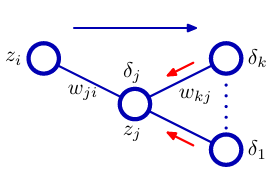
\includegraphics[width=0.3\linewidth]{img/aprendizajegd.png}
    \caption[Proceso de retropropagación del error~\cite{Bishop2006}.]{Proceso de retropropagación del error~\cite{Bishop2006}. Dado un lote de entrenamiento, se propaga la información hacia delante (flecha azul), se calculan las activaciones y el error de salida. Seguidamente, se realiza el paso hacia atrás (flechas rojas), calculando el error $\delta_j$ de cada unidad $j$ en cada capa. Finalmente, se actualizan los parámetros utilizando el gradiente calculado.}\label{fig:aprendizajegd}
\end{figure}

Una vez obtenida la predicción, se calcula la función de pérdida para evaluar la discrepancia entre la predicción y el valor real. De esta manera, podemos describir la salida resultante de cualquier neurona mediante la siguiente expresión, extraída de~\cite{Prince2023}:

\begin{equation}
    h_d = \phi \left( w_{d0} + \sum_{i=1}^{D_i} w_{di} x_i \right)
    \label{eq:hidden_unit}
\end{equation}

donde $d$ hace referencia a la neurona en dicha posición, $\phi$ representa una función de activación no lineal, $x_i \in \mathbb{R}^{D_i}$ representa la entrada multidimensional, donde $D_i$ es el número de características de entrada (en este caso consideramos nuestro conjunto de datos de entrenamiento $\mathcal{D}$ como un subconjunto de $\mathbb{R}^{D_i}$) y $w_{di}$ con $i \in \{0,1,\ldots,D_i\}$ representa los pesos que conectan la entrada $x_i$ con la neurona $d$, donde para $i = 0$ se obtiene el término del sesgo.\newline

Seguidamente, se inicia la segunda fase del aprendizaje, cuyo objetivo es ajustar los parámetros de la red para minimizar ese error. Para ello, se utiliza retropropagación del error o \emph{backpropagation}, que calcula el gradiente de la función de pérdida con respecto a los pesos y sesgos, mediante la regla de la cadena del cálculo diferencial. Posteriormente, el algoritmo de descenso de gradiente actualiza los pesos en la dirección opuesta al gradiente.\newline

En conlusión, el forward pass y la backpropagation trabajan de manera conjunta para permitir que la red neuronal aprenda de manera efectiva. El forward pass genera las predicciones para los datos de entrada, la función de pérdida evalúa el error cometido en dichas predicciones, la backpropagation calcula la contribución de cada unidad a dicho error (véase~\autoref{fig:aprendizajegd}) y, por último, el descenso de gradiente ajusta los parámetros para mejorar las predicciones futuras, repitiéndose este ciclo a lo largo de múltiples iteraciones.\newline

\section{Bias-variance tradeoff}\label{sec:capitulo-bias-variance-tradeoff}
El objetivo del aprendizaje radica en obtener un bajo error de prueba o generalización ($E_{out}$) sobre datos desconocidos, lo que implicará que hemos conseguido aproximar de buena manera la función objetivo $f$. La capacidad para conseguir un bajo error de generalización está ligada directamente al conjunto de hipótesis ($\mathcal{H}$), donde si nuestro conjunto es suficientemente grande tendremos una mayor probabilidad de aproximar la función objetivo $f$, al disponer de un mayor número de funciones candidatas. Sin embargo, si nuestro conjunto $\mathcal{H}$ es demasiado grande, puede darse el caso de que, al elegir una de las funciones candidatas (usando nuestro conjunto de entrenamiento), dicha función no sea la que mejor aproxime a la función objetivo, lo que provoque un mayor error de generalización. A este problema se le conoce como el problema del \textit{equilibrio entre aproximación y generalización}. Adicionalmente, el conjunto de hipótesis ideal sería el formado únicamente por la función objetivo, es decir, $\mathcal{H} = \{f\}$.\newline

El análisis sesgo-varianza o \emph{bias-variance analysis} busca descomponer el error de generalización en dos términos principales:

\begin{enumerate}
    \item Cómo de bien puede $\mathcal{H}$ aproximar a la función objetivo $f$ en general, no solo en la muestra.
    \item Hasta qué punto podemos acercanos a una buena función candidata $g \in \mathcal{H}$.\newline
\end{enumerate}

Adicionalmente, el error de generalización $E_{out}$ incluye un término adicional conocido como \textit{ruido}. Este término hace referencia al error irreducible que se encuentra de manera natural en los datos y que, generalmente, es debido a factores fuera del control del modelo, tales como mediciones imprecisas o variables no modeladas. Dado que este tipo de error es inevitable y no puede ser reducido, no se considera relevante en la descomposición del error. Sin embargo, cabe destacar que este ruido suele ser una limitación fundamental de la generalización del modelo.\newline

\subsection{Formulación matemática del $E_{out}$}\label{sec:formulacion-matematica-Eout}
A continuación, detallaremos matemáticamente las componentes del error fuera de la muestra o de generalización. Para ello y con objeto de simplificar la descomposición del $E_{out}$ de manera limpia en los dos términos principales citados anteriormente, vamos a considerar un problema de regresión que no presenta ruido en los datos, utilizando el error cuadrático como medida de evaluación del error.\newline

Sea $g^{\mathcal{(D)}} \in \mathcal{H}$ nuestra función candidata elegida (hipótesis final), que dependerá del conjunto de datos utilizado ($\mathcal{D}$). Destacamos que, dado cualquier otro conjunto de datos, encontraremos una hipótesis final distinta.\newline

El \emph{error de generalización o error fuera de la muestra}, definido como la diferencia entre la predicción del modelo y los valores reales en un conjunto de datos no visto durante el entrenamiento, quedaría expresado de la siguiente forma:
\begin{equation}\label{eq:E_out1}
    E_{out}(g^{\mathcal{(D)}}) = \mathbb{E}_{x}[{(g^{\mathcal{(D)}}(x) - f(x))}^2], \quad x \notin \mathcal{D}
\end{equation}

donde $\mathbb{E}_{x}$ denota el valor esperado con respecto a $x$ (basado en la distribución de probabilidad del espacio de entrada $\mathcal{X})$, con el objetivo de obtener el valor esperado del error en todo el espacio.\newline

Dado que la ecuación~\eqref{eq:E_out1} depende de un conjunto de datos en particular, podemos eliminar esta dependencia del conjunto de datos utilizado tomando el valor esperado de dicho error con respecto a todos los conjuntos de datos:

\begin{equation}\label{eq:E_out2}
    \mathbb{E}_{\mathcal{D}}[E_{out}(g^{\mathcal{(D)}})] = \mathbb{E}_{\mathcal{D}}[\mathbb{E}_{x}[{(g^{\mathcal{(D)}}(x) - f(x))}^2]]. 
\end{equation}\newline

Cambiamos ahora el orden de las esperanzas dado que, en realidad, estamos integrando y cambiando el orden de integración, que podemos realizarlo dado que el integrando ${(g^{\mathcal{(D)}}(x) - f(x))}^2$ es estrictamente no negativo:

\begin{equation}\label{eq:E_out3}
    \mathbb{E}_{\mathcal{D}}[E_{out}(g^{\mathcal{(D)}})] = \mathbb{E}_{x}[\mathbb{E}_{\mathcal{D}}[{(g^{\mathcal{(D)}}(x) - f(x))}^2]].
\end{equation}\newline

Nos centramos en calcular $\mathbb{E}_{\mathcal{D}}[{(g^{\mathcal{(D)}}(x) - f(x))}^2]$, olvidándonos por ahora del valor esperado sobre $x$, dado que nos interesa calcular la esperanza con respecto a $\mathcal{(D)}$ hasta obtener una descomposición limpia del error. Para ello, vamos a definir el concepto de hipótesis promedio $\bar{g}(x)$ de la siguiente manera:

\begin{equation}\label{eq:gbar}
    \bar{g}(x) = \mathbb{E}_{\mathcal{D}}[g^{\mathcal{(D)}}(x)]
\end{equation}

que corresponde al valor esperado de todas las hipótesis que podemos obtener al aprender de los distintos conjuntos de datos que utilicemos. Destacamos que, en la ecuación~\eqref{eq:gbar}, tenemos $x$ (punto de prueba) fijo, por lo que $g^{\mathcal{(D)}}(x)$ es una variable aleatoria determinada por la elección de nuestros datos, donde si tomamos distintos conjuntos de datos, obtendremos distintos valores para la hipótesis en el punto $x$ fijado. Sin embargo, en la realidad nunca dispondremos de esta hipótesis promedio, pues tendríamos un número infinito de conjuntos de datos distintos. Además, cabe destacar que la hipótesis promedio no tiene asegurada su pertenencia al conjunto de hipótesis $\mathcal{(H)}$, aunque sea el promedio de hipótesis pertenecientes a $\mathcal{H}$.\newline

Continuando con la descomposición, tenemos el siguiente resultado:

\begin{equation}\label{eq:E_out4}
    \mathbb{E}_{\mathcal{D}}[{(g^{\mathcal{(D)}}(x) - f(x))}^2] = \mathbb{E}_{\mathcal{D}}[{(g^{\mathcal{(D)}}(x) - \bar{g}(x) + \bar{g}(x) - f(x))}^2]
\end{equation}

donde se ha sumado y restado la misma cantidad ($\bar{g}(x)$) para simplificar la descomposición.\newline

Seguidamente, continuamos desarrollando el término cuadrático de la ecuación~\eqref{eq:E_out4}:

\[ \mathbb{E}_{\mathcal{D}}[{(g^{\mathcal{(D)}}(x) - \bar{g}(x))}^2 + {(\bar{g}(x) - f(x))}^2 + 2(g^{\mathcal{(D)}}(x) - \bar{g}(x))(\bar{g}(x) - f(x))]. \]\newline

Dado que estamos realizando el valor esperado con respecto a $\mathcal{D}$, de la ecuación anterior tenemos que $(\bar{g}(x) - f(x))$ es una constante. Por tanto, dado que el valor esperado de una constante es la propia constante, para obtener el valor esperado del término cruzado solo necesitamos conocer el valor esperado de $(g^{\mathcal{(D)}}(x) - \bar{g}(x))$:

\begin{equation}\label{eq:E_out6}
    \mathbb{E}_{\mathcal{D}}[g^{\mathcal{(D)}}(x) - \bar{g}(x)] = \mathbb{E}_{\mathcal{D}}[g^{\mathcal{(D)}}(x)] - \mathbb{E}_{\mathcal{D}}[\bar{g}(x)] = \bar{g}(x) - \bar{g}(x) = 0.
\end{equation}\newline

Finalmente, de la ecuación~\eqref{eq:E_out4} nos queda la siguiente expresión:

\begin{equation}\label{eq:E_out7}
    \mathbb{E}_{\mathcal{D}}[{(g^{\mathcal{(D)}}(x) - f(x))}^2] = \mathbb{E}_{\mathcal{D}}[{(g^{\mathcal{(D)}}(x) - \bar{g}(x))}^2] + {(\bar{g}(x) - f(x))}^2
\end{equation}

donde hemos usado que el valor esperado de una constante $(\bar{g}(x) - f(x))$ es igual a dicha constante.\newline

Por consiguiente, hemos obtenido una descomposición de la ecuación~\eqref{eq:E_out4} en dos términos que serán los asociados a los términos de varianza (\textit{variance}) y sesgo (\textit{bias}) respectivamente.

\begin{enumerate}
    \item $\mathbb{E}_{\mathcal{D}}[{(g^{\mathcal{(D)}}(x) - \bar{g}(x))}^2]$: nos indica cómo de lejos se encuentra nuestra hipótesis, $g^{\mathcal{(D)}}(x)$, obtenida de un conjunto de datos particular de la mejor (promedio) hipótesis, $\bar{g}(x)$, que podemos obtener utilizando nuestro conjunto de hipóstesis $\mathcal{H}$. Este es el término asociado a la varianza de $x$ ($\textbf{var(x)}$).
    \item ${(\bar{g}(x) - f(x))}^2$: nos indica cómo de lejos se encuentra dicha hipótesis ideal, $\bar{g}(x)$, de la función objetivo $f(x)$. Este es el término asociado al sesgo de $x$ ($\textbf{bias(x)}$).\newline
\end{enumerate}

Por tanto, volviendo a la ecuación~\eqref{eq:E_out3} nos queda:

\begin{equation}\label{eq:E_out8}
    \mathbb{E}_{\mathcal{D}}[E_{out}(g^{\mathcal{(D)}})] = \mathbb{E}_{x}[\mathbb{E}_{\mathcal{D}}[{(g^{\mathcal{(D)}}(x) - f(x))}^2]] = \mathbb{E}_{x}[\textbf{var(x)} + \textbf{bias(x)}]
\end{equation}

donde denotaremos por \textbf{sesgo} a $\mathbb{E}_{x}[\textbf{bias(x)}]$ y por \textbf{varianza} a $\mathbb{E}_{x}[\textbf{var(x)}]$.\newline

\begin{observacion}
    Cuando hay ruido presente en los datos de entrenamiento, es decir, $y(x) = f(x) + \epsilon(x)$ y, además, $\epsilon$ es una variable aleatoria con media $0$ y varianza $\sigma^{2}$, entonces

    \[ E_{out}(g^{(\mathcal{D})}) = \mathbb{E}_{x, y}[g^{(\mathcal{D})}(x)-{y(x)}^{2}] \]

    y, en este caso, se verifica

    \[ \mathbb{E}_{\mathcal{D}}[E_{out}(g^{(\mathcal{D})})] = \sigma^{2} + bias + var. \]
\end{observacion}

\begin{proof}
    Dado que asumimos que $\epsilon$ es una variable aleatoria con media $0$, obtenemos que $\mathbb{E}[\epsilon(x)] = 0$.

    \begin{equation}\label{eq:E_out-noise1}
        \mathbb{E}_{\mathcal{D}, \epsilon}[{(g^{\mathcal{(D)}}(x) - y(x))}^2] = \mathbb{E}_{\mathcal{D}, \epsilon}[{(g^{\mathcal{(D)}}(x) - f(x)) - \epsilon(x)}^2]
    \end{equation}

    donde dado que $y$ depende del ruido, consideramos también el valor esperado con respecto a $\epsilon$ que afectará únicamente a $y$. Procediendo de manera similiar a la Ecuación~\eqref{eq:E_out4}, obtenemos

    \begin{equation}
        \mathbb{E}_{\mathcal{D}, \epsilon}[{(g^{\mathcal{(D)}}(x) - \bar{g}(x) + \bar{g}(x) - f(x) - \epsilon(x))}^2]
    \end{equation}

    y, tras realizar operaciones, llegamos a

    \begin{equation}
        \mathbb{E}_{\mathcal{D}, \epsilon}[{(g^{\mathcal{(D)}}(x) - f(x))}^2] + 2\mathbb{E}_{\mathcal{D}, \epsilon}[(g^{\mathcal{(D)}}(x)-f(x))\epsilon(x)] + \mathbb{E}_{\mathcal{D}, \epsilon}[\epsilon^{2}(x)]
    \end{equation}

    donde el primer sumando no depende de $\epsilon$, el tercer sumando no depende de $\mathcal{D}$ y el segundo sumando puede expresarse de la siguiente forma:

    \begin{equation}
        2\mathbb{E}_{\mathcal{D}, \epsilon}[(g^{\mathcal{(D)}}(x)-f(x))\epsilon(x)] = 2\mathbb{E}_{\mathcal{D}, \epsilon}[(g^{\mathcal{(D)}}(x)-f(x))]\mathbb{E}_{\mathcal{D}, \epsilon}[\epsilon(x)].
    \end{equation}

    donde el valor esperado con respecto a $\epsilon$ no depende de $\mathcal{D}$. De esta manera y conociendo que $\mathbb{E}_{\epsilon}[\epsilon(x)] = 0$ y $\mathbb{E}_{\epsilon}[{\epsilon(x)}^{2}] = \sigma^{2}$, obtenemos que la Ecuación~\eqref{eq:E_out-noise1} puede expresarse de la siguiente forma

    \begin{equation}
        \mathbb{E}_{\mathcal{D}, \epsilon}[{(g^{\mathcal{(D)}}(x) - y(x))}^2] = \mathbb{E}_{\mathcal{D}}[{(g^{\mathcal{(D)}}(x) - f(x))}^2] + \sigma^{2}.
    \end{equation}

    Finalmente, aplicando el valor esperado sobre $x$ a la expresión anterior, obtenemos el resultado buscado.\newline
\end{proof}

Como conclusión de esta sección, detallaremos algunos aspectos clave del análisis del sesgo y de la varianza:

\begin{itemize}
    \item Aunque el análisis de sesgo-varianza se basa en la medida del error cuadrático, el algoritmo de aprendizaje utilizado por el modelo no tiene que basarse en minimizar el error cuadrático. Es decir, se puede usar cualquier otro criterio (función de pérdida) para producir $g^{\mathcal{(D)}}$ basado en el conjunto de datos $\mathcal{D}$ y, una vez que tenemos $g^{\mathcal{(D)}}$, calculamos su sesgo y varianza utilizando el error cuadrático.
    \item El sesgo y la varianza no pueden ser calculados en la práctica, ya que dependen de la función objetivo y de la distribución de probabilidad de la entrada (ambas desconocidas), por lo que su descomposición resulta de utilidad como una herramienta conceptual a la hora de entender y desarrollar un modelo.\newline
    
\end{itemize}

\section{Equilibrio clásico entre sesgo y varianza}\label{sec:equilibrio-sesgo-varianza}
Siguiendo con los resultados obtenidos en la \autoref{sec:formulacion-matematica-Eout}, nuestro objetivo ahora es minimizar el error fuera de la muestra, inducido por tres componentes: ruido, sesgo y varianza. Dado que, como se ha comentado previamente, el rudio es irreducible y no hay nada que podamos hacer para evitarlo, nos centraremos en intentar reducir los dos términos principales reducibles del error: el sesgo y la varianza.\newline

Conocemos que el sesgo viene definido por la medida en la que la predicción ideal obtenida de todos los conjuntos de datos difiere de la función objetivo, o expresado de manera similar, el sesgo es el resultado de la incapacidad del modelo para describir la función objetivo. Este resultado sugiere que podemos reducir este término de error haciendo que nuestro modelo sea más flexible, es decir, aumentando nuestro conjunto de hipótesis $\mathcal{H}$ (haciéndolo más complejo), con el objetivo de disponer de un mayor número de funciones candidatas para forzar que la hipótesis promedio se aproxime lo máximo posible a la función objetivo.\newline

Por otro lado, la varianza viene a ofrecernos la medida en la que varían las hipótesis para distintos conjuntos de datos con respecto a la hipótesis ideal, o expresado de manera similar, la varianza evalúa cómo de sensible es una hipótesis a la selección específica del conjunto de datos $\mathcal{D}$. Este análisis revela que podemos reducir este término de error disminuyendo el conjunto de hipótesis ya que, en un espacio de hipótesis restringido, al haber menos hipótesis, las hipótesis son menos sensibles a las variaciones en el conjunto de datos. Como resultado, al cambiar el conjunto de datos para seleccionar una hipótesis, es más probable que se elijan hipótesis similares.\newline

En consecuencia, observamos una dependencia de ambos términos de error con respecto a la complejidad del conjunto de hipótesis ($\mathcal{H}$) utilizado. Esta dependencia viene dada por:

\begin{itemize}
    \item Al aumentar la complejidad del conjunto de hipótesis, es decir, al incrementar su tamaño, el sesgo disminuirá, pero la varianza irá aumentado.
    \item Si reducimos la complejidad del conjunto de hipótesis, es decir, disminuimos su tamaño, el sesgo irá aumentando, pero la varianza disminuirá.\newline
\end{itemize}

De este modo, el equilibrio buscado en esta sección con objeto de minimizar el error fuera de la muestra viene ligado a la elección de un conjunto de hipótesis ($\mathcal{H}$) suficientemente complejo como para acercanos a la función objetivo y suficientemente simple como para no disponer de una cantidad excesiva de hipótesis que induzcan un alto grado de varianza. Este equilibrio se podrá conseguir mediante diversas técnicas, como la regularización, que se explicarán en secciones posteriores.\newline

\begin{figure}[h]
    \centering
    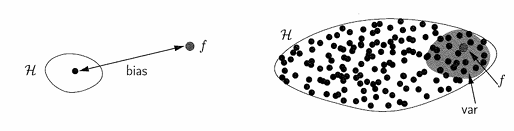
\includegraphics[width=0.7\linewidth]{img/bias-variance.png}
    \caption[Distintos casos del conjunto de hipótesis y de la función objetivo.] {Distintos casos del conjunto de hipótesis y de la función objetivo~\cite{Mostafa2012}. A la izquierda observamos como nuestro conjunto de hipótesis presenta únicamente una función candidata, alejada de la función objetivo $f$, lo que implica un alto sesgo y una varianza nula. A la derecha observamos un conjunto de hipótesis con numerosas funciones candidatas que incluye a la función objetivo $f$, por lo que el sesgo es muy cercano a $0$ y la varianza es grande.}\label{fig:bias-variance}
\end{figure}

\subsection{Curva de aprendizaje}

Para finalizar este capítulo, introduciremos el concepto de curva de aprendizaje o \emph{learning curve}, que será la principal herramienta que utilizaremos a lo largo de todo el proyecto para analizar el rendimiento de los distintos modelos que utilicemos.\newline

En primer lugar y de manera análoga a la ecuación~\eqref{eq:E_out1}, definimos el \emph{error de entrenamiento o error dentro de la muestra ($E_{in}$)} como la diferencia entre la predicción del modelo y los valores reales del conjunto de datos de entrenamiento, es decir

\begin{equation}\label{eq:E_in1}
    E_{in}(g^{\mathcal{(D)}}) = \mathbb{E}_{x}[{(g^{\mathcal{(D)}}(x) - f(x))}^2], \quad x \in \mathcal{D}.
\end{equation}\newline

Por consiguiente, después de aprender de un conjunto particular de datos $\mathcal{D}$ de tamaño $N$, la hipótesis final elegida $g^{(\mathcal{D})}$ tendrá error de entrenamiento ($E_{in}(g^{(\mathcal{D})})$) y error de generalización ($E_{out}(g^{(\mathcal{D})})$), ambos dependiendo del conjunto de datos utilizado. Como se comentó en la \autoref{sec:formulacion-matematica-Eout}, al realizar la esperanza con respecto a todos los conjuntos de datos de dichos errores obtenemos los errores esperados $\mathbb{E}_{\mathcal{D}}[E_{in}(g^{(\mathcal{D})})]$ y $\mathbb{E}_{\mathcal{D}}[E_{out}(g^{(\mathcal{D})})]$, donde ambos errores son funciones del tamaño del conjunto de datos ($N$).\newline

\begin{figure}[h]
    \centering
    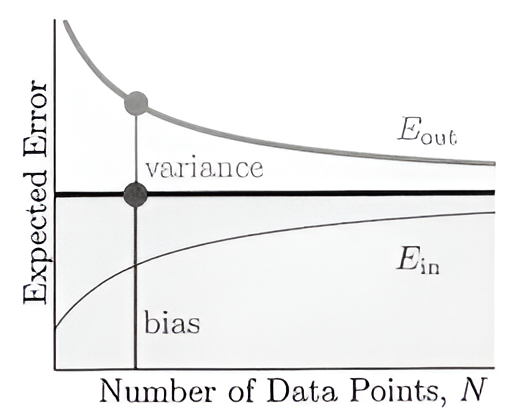
\includegraphics[width=0.4\linewidth]{img/learning-curve.png}
    \caption[Ejemplo de curva de aprendizaje tradicional~\cite{Mostafa2012}.] {Ejemplo de curva de aprendizaje tradicional~\cite{Mostafa2012}. Observamos la curva de aprendizaje de un modelo con respecto al tamaño del conjunto de datos. Se puede comprobar como el $E_{out}$ decrece, mientras que el $E_{in}$ crece. Además, se puede apreciar la descomposición sesgo-varianza, donde la línea central en negrita denota la hipótesis promedio.}\label{fig:learning-curve-bias-variance}
\end{figure}

Denominaremos \emph{curva de aprendizaje} a la representación gráfica que muestra la relación entre el rendimiento de un modelo y el tamaño del conjunto de datos utilizado para su entrenamiento, es decir, a la gráfica que incluye los errores esperados $\mathbb{E}_{\mathcal{D}}[E_{in}(g^{(\mathcal{D})})]$ y $\mathbb{E}_{\mathcal{D}}[E_{out}(g^{(\mathcal{D})})]$ como función de $N$.\newline

Además, dado que la curva de aprendizaje está ligada a los errores esperados del modelo tanto dentro como fuera de la muestra, podríamos analizar el equilibrio sesgo-varianza directamente sobre dicha gráfica. Sin embargo, para llevar a cabo dicho análisis, necesitaríamos conocer la hipótesis promedio $\bar{g}$ que, como sabemos de secciones anteriores, es imposible de calcular. No obstante, si tuvieramos dicha hipótesis promedio, podríamos realizar el análisis (véase \autoref{fig:learning-curve-bias-variance}), teniendo en cuenta que el $E_{out}$ es suma de sesgo y varianza (obviando el término de ruido).\newline

Sin embargo, de cara a analizar el doble descenso a lo largo del proyecto, \textbf{no utilizaremos directamente la curva de aprendizaje} tal y como se ha definido, dado que nuestro objetivo es analizar el error con respecto a la capacidad del modelo y no en función del número de datos utilizados. Es por esto que, nuestra curva de aprendizaje será una modificación de la curva de aprendizaje original, donde en el eje $X$ de la gráfica aparecerá indistintamente la capacidad o el número de épocas de entrenamiento del modelo y en el eje $Y$ el error esperado (véase~\autoref{fig:learning-curve-classicalvsmodern}), tanto dentro como fuera de la muestra, para un número fijo de datos de entrenamiento.\newline

\begin{figure}[h]
    \centering
    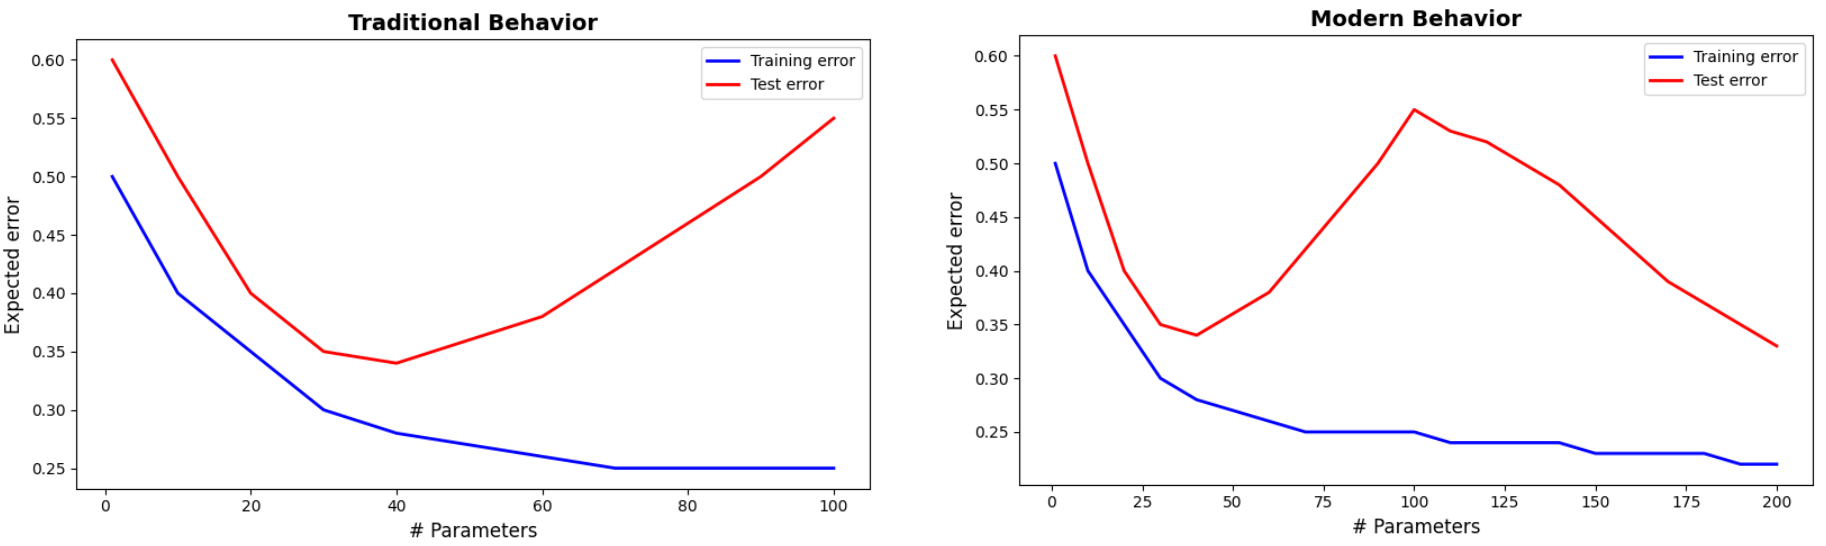
\includegraphics[width=0.9\linewidth]{img/learning-curve-classicalvsmodern.png}
    \caption[Ejemplos de curvas de aprendizaje modificadas para este proyecto.] {Ejemplos de curvas de aprendizaje modificadas para este proyecto. A la izquierda se muestra la curva clásica de aprendizaje, donde el error de test aumenta llegado a un cierto punto. A la derecha, la curva moderna refleja que, al aumentar la complejidad del modelo más allá de lo establecido en la sabiduría clásica, el error de test vuelve a disminuir. Imagen original del autor.}\label{fig:learning-curve-classicalvsmodern}
\end{figure}

\section{Underfitting y overfitting}\label{sec:subsec-underfitting-y-overfitting}

Consideremos nuevamente el problema del aprendizaje supervisado que estamos tratando, consistente en encontrar una ``buena'' función aproximadora $g \in \mathcal{H}$ basada en los datos de un determinado conjunto de entrenamiento $\mathcal{D}$. Además, se asume que estos datos provienen de una determinada distribución de probabilidad, es decir, $\mathcal{D} = \{(X_{1}, Y_{1}), \ldots, (X_{n}, Y_{n})\}$ es una colección de $n$ copias idénticas e idénticamente distribuidas de las variables aleatorias $(X, Y)$ que toman valores en $\mathcal{X} \times \mathcal{Y}$ y que siguen una distribución de probabilidad conjunta $P[X, Y]$, permitiendo modelar la incertidumbre en las predicciones. De igual manera, se asume la existencia de una función real no negativa $L(g(X), Y)$, denominada $\textit{función de pérdida}$, que es la encargada de evaluar la diferencia entre la predicción realizada por la función candidata $g$ y el verdadero valor $y$.\newline

En lo que prosigue a lo largo de esta sección, restringiremos nuestro conjunto de hipótesis $\mathcal{H}$ a una determinada clase de funciones, es decir, $\mathcal{H}$ quedaría fijo y trabajaremos en el contexto de la sabiduría tradicional, es decir, cuando el número de parámetros del modelo es significativamente menor que el número de datos de entrenamiento disponibles.\newline

\begin{definicion}[Riesgo real]\label{def:riesgo-real}
    El riesgo real asociado a la función candidata $g \in \mathcal{H}$ viene definido como el valor esperado de la función de pérdida, esto es

    \[ L(g) = \mathbb{E}[L(g(X), Y)] = \int_{\mathcal{X}} L(g(X), Y) \, dP[X, Y] = P[g(X) \neq Y].\]

    El riesgo real es también denominado como $\textit{error de generalización}$.\newline
\end{definicion}

Por tanto, el objetivo final de un algoritmo de aprendizaje, como se comentó en secciones anteriores, es encontrar la función candidata $g^{*}$ entre una clase fija de funciones del conjunto de hipótesis $\mathcal{H}$ para la cual el riesgo real sea mínimo, es decir

\[ g^{*} = \operatorname*{\arg \,\min}_{g \in \mathcal{H}} L(g). \]\newline

No obstante, en la práctica y por lo general, el riesgo real no puede ser calculado porque la distibución conjunta P[X, Y] es desconocida por el algoritmo de aprendizaje. Es por esto que tenemos que recurrir a un cálculo estimado del mismo, denominado $\textit{riesgo empírico}$, calculado haciendo uso de la media de la función de pérdida sobre el conjunto de entrenamiento.\newline

\begin{definicion}[Riesgo empírico]\label{def:riesgo-empírico}
    El riesgo empírico asociado a la función candidata $g \in \mathcal{H}$ sobre el conjunto de entrenamiento $\mathcal{D}$ viene definido por

    \[ L_{emp}(g) = \frac{1}{n} \sum_{i=1}^{n}L(g(X_{i}), Y_{i}). \]\newline
\end{definicion}

Ligado a este concepto surge el $\textit{principio de minimización del riesgo empírico}$ \cite{Vapnik1991}, que establece que el algoritmo de aprendizaje $\mathcal{A}$ debe elegir una función candidata $\hat{g}$ sobre el conjunto de hipótesis $\mathcal{H}$ que minimice el riesgo empírico sobre el conjunto de entrenamiento $\mathcal{D}$, es decir

\begin{equation}\label{eq:riesgo-empirico}
    \hat{g} = \operatorname*{\arg \,\min}_{g \in \mathcal{H}} L_{emp}(g). 
\end{equation}\newline

Finalmente, la diferencia entre cualquier función candidata $g \in \mathcal{H}$ y la mejor función candidata $g^{*}$ puede descomponerse de la siguiente manera~\cite{Lafon2024}:

\[
L(g) - L(g^{*}) = \underbrace{L(g) - \inf_{g \in \mathcal{H}} L(g)}_{\text{error de estimación}} + \underbrace{\inf_{g \in \mathcal{H}} L(g) - L(g^{*})}_{\text{error de aproximación}}
\]

donde, aparte del error de estimación y del error de aproximación, existe otra fuente de error conocida como $\textit{error de optimización}$ que indica la diferencia entre el riesgo de la función candidata, devuelto por el procedimiento de optimización (en nuestro caso el descenso de gradiente), y un minimizador del riesgo empírico. De esta manera, el algoritmo de aprendizaje $\mathcal{A}$ definido por el principio de minimización del riesgo empírico consiste en resolver el problema de optimización dado por la ecuación~\eqref{eq:riesgo-empirico}.\newline

\begin{proposicion}\label{prop:min-riesgo-empirico}
    Para cualquier minimizador del riesgo empírico $\hat{g}$, el error de estimación verifica

    \[ L(\hat{g}) - \inf_{g \in \mathcal{H}}L(g) \leq 2 \sup_{g \in \mathcal{H}}|L_{emp}(g) - L(g)|. \]\newline
\end{proposicion}

\begin{proof}
    Partimos de la siguiente desigualdad

    \[ L(\hat{g}) - \inf_{g \in \mathcal{H}}L(g) \leq  |L(\hat{g}) - L_{emp}(\hat{g})| + |L_{emp}(\hat{g}) - \inf_{g \in \mathcal{H}}L(g)| \]

    con el primer sumando verificando

    \[ |L(\hat{g}) - L_{emp}(\hat{g})| \leq \sup_{g \in \mathcal{H}}|L_{emp}(g) - L(g)|\]

    dado que $\hat{g} \in \mathcal{H}$. Por otra parte, el segundo sumando verifica

    \[ |L_{emp}(\hat{g}) - \inf_{g \in \mathcal{H}}L(g)| = |\inf_{g \in \mathcal{H}} L_{emp}(g) - \inf_{g \in \mathcal{H}}L(g)| \leq \sup_{g \in \mathcal{H}}|L_{emp}(g) - L(g)| \]

    y, sumando ambas desigualdades, se obtiene el resultado deseado.\newline
\end{proof}

De este modo, la estrategia a seguir en el aprendizaje automático es la de encontrar un correcto conjunto de hipótesis $\mathcal{H}$ para mantener ambos errores lo más pequeños posible. Es por esto que, dependiendo del conjunto $\mathcal{H}$ elegido, podemos encontrarnos las siguientes situaciones:

\begin{enumerate}
    \item Si el conjunto $\mathcal{H}$ es muy ``pequeño'', ninguna función candidata será capaz de capturar la complejidad de los datos de entrenamiento y no será capaz de aproximarse a $g^{*}$. A esta situación la llamaremos subajuste o \emph{underfitting}.
    \item Si el conjunto $\mathcal{H}$ es muy ``grande'', el límite de la Proposición~\ref{prop:min-riesgo-empirico} (máxima brecha de generalización sobre $\mathcal{H}$) aumentará y la función candidata $\hat{g}$ elegida como minimizadora del riesgo empírico puede generalizar de forma no adecuada aún teniendo un error de entrenamiento bajo. A esta situación la llamaremos sobreajuste o \emph{overfitting}.
\end{enumerate}

Como conclusión de estas situaciones, se pone de manifiesto la fuerte dependencia de la minimización empírica del riesgo (error del modelo) del conjunto de hipótesis elegido. Además, es posible establecer de manera clara la relación entre la descomposición del error de generalización como suma de sesgo y varianza y los fenómenos de \emph{underfitting} y \emph{overfitting} (véase Figura~\ref{fig:biasvarianceunderoverfitting}). De esta manera, cuando el modelo se encuentra en la zona de subajuste, su estructura es demasiado simple y no logra capturar los patrones presentes en los datos. Esto se traduce en un error elevado tanto en el conjunto de entrenamiento como en el de prueba, ligado a un alto sesgo. Por otro lado, cuando el modelo se encuentra en la zona de sobreajuste, se ajusta en exceso a los datos de entrenamiento, llegando a memorizar el ruido. En este caso, el modelo presenta un desempeño prácticamente perfecto en el conjunto de entrenamiento, pero su capacidad de generalización a nuevos datos es deficiente, ligado a una varianza elevada y un sesgo bajo.\newline

\begin{figure}[h]
    \centering
    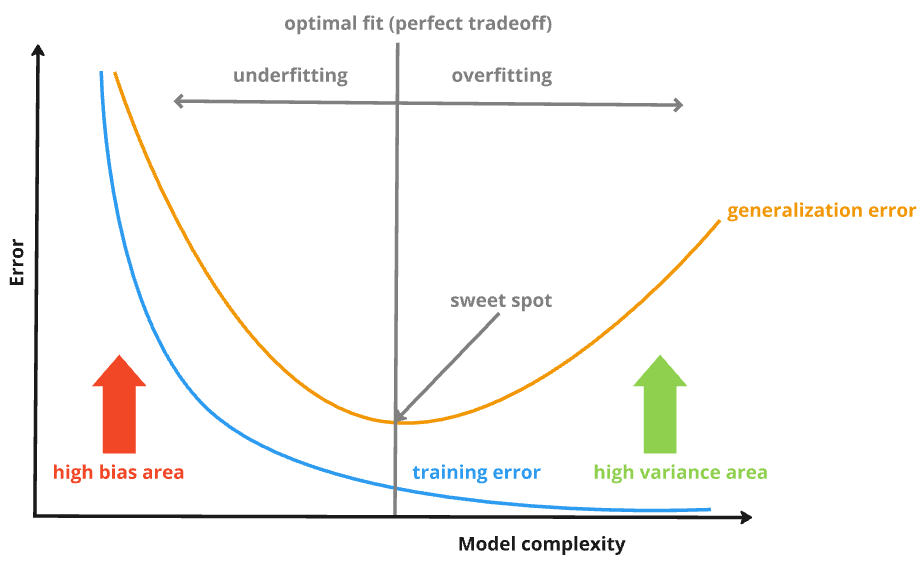
\includegraphics[width=0.8\linewidth]{img/biasvarianceunderoverfitting.png}
    \caption[Relación bias/variance con underfitting y overfitting en el contexto clásico.] {Relación bias/variance con underfitting y overfitting en el contexto clásico. Al principio, el modelo muestra un alto sesgo, incapaz de capturar adecuadamente las relaciones entre los datos. A medida que aumenta su complejidad, tanto el rendimiento en entrenamiento como en test mejora, alcanzando un punto de equilibrio en el mínimo de la curva del error de generalización (\textit{sweet spot}). Al superar este punto óptimo, el modelo comienza a memorizar los datos, lo que provoca un aumento del error de generalización, ligado a una mayor varianza. Imagen original del autor.}\label{fig:biasvarianceunderoverfitting}
\end{figure}

En definitiva, para minimizar el error de generalización en la zona clásica, es fundamental encontrar un equilibrio entre sesgo y varianza, evitando tanto el \emph{underfitting} como el \emph{overfitting}. Este equilibrio se logra mediante una elección adecuada del conjunto de hipótesis $\mathcal{H}$, el cual debe ser lo suficientemente expresivo para capturar patrones relevantes en los datos sin llegar a ser demasiado complejo para que termine modelando el ruido presente en los mismos.

\endinput
